% !TEX program = lualatex
\documentclass[12pt,a4paper]{article}
\usepackage{fontspec}
\setmonofont{Latin Modern Mono}
\usepackage{xcolor}
\usepackage{listings}
\usepackage{geometry}
\usepackage{fancyhdr}
\usepackage{hyperref}
\usepackage{graphicx}
\geometry{margin=1in}
\usepackage{multicol}

% -------------------------------
% SOLUTION TOGGLE
% -------------------------------
\newif\ifshowsolutions
\showsolutionstrue 
% \showsolutionsfalse

% -------------------------------
% Header and Footer Configuration
% -------------------------------
\pagestyle{fancy}
\fancyhf{}
\lhead{Lab Final}
\rhead{CSE 4308: DBMS Lab}
\cfoot{\thepage}
\setlength{\headwidth}{\textwidth}

% -------------------------------
% Code Listing Style
% -------------------------------
\definecolor{codegreen}{rgb}{0,0.6,0}
\definecolor{codegray}{rgb}{0.5,0.5,0.5}
\definecolor{codepurple}{rgb}{0.58,0,0.82}
\definecolor{backcolour}{rgb}{0.95,0.95,0.92}

\lstdefinestyle{mystyle}{
    backgroundcolor=\color{backcolour},
    commentstyle=\color{codegreen},
    keywordstyle=\color{magenta},
    numberstyle=\tiny\color{codegray},
    stringstyle=\color{codepurple},
    basicstyle=\ttfamily\footnotesize,
    breaklines=true,
    captionpos=b,
    keepspaces=true,
    numbers = none,
    numbersep=5pt,
    tabsize=2,
    frame=single,
    columns=fullflexible,
    showspaces=false,
    showstringspaces=false,
    showtabs=false
}

\lstset{style=mystyle}

% Images: found next to this file (local compile_labs.sh) or via the
% lab folder when compiled from the project root (Overleaf).
\graphicspath{{lab_14_final/}}

\begin{document}

% --------------------------------------------------------------
% TITLE PAGE
% --------------------------------------------------------------
\begin{titlepage}
    \centering
    \vspace*{2\baselineskip}

    \rule{14cm}{2pt}\vspace*{-0.8\baselineskip}\vspace*{1.5pt}
    \rule{14cm}{0.5pt}\vspace{2\baselineskip}

    {\Huge\bfseries\scshape Lab Final\par}
    \vspace{3mm}
    {\Large }
    \vspace{3mm}

    \rule{14cm}{0.5pt}\vspace*{-0.7\baselineskip}\vspace{2.5pt}
    \rule{14cm}{2pt}

    \vspace{2\baselineskip}

    {\Large\bfseries CSE 4308\par}
    \vspace{1\baselineskip}
    {\large DATABASE MANAGEMENT SYSTEMS LAB\par}

    \vfill
    {\normalsize Prepared by:\\ Samnun Azfar, Jr. Lecturer, CSE\\ Samia Nawsheen, Jr. Lecturer, CSE\par}
    {\normalsize Academic Year: AY25-26\par}
\end{titlepage}

\newpage
\newpage

% ==============================================================
\section{Lab Final}


\begin{enumerate}

% ==============================================================

% ==============================================================
% \item List the \texttt{film\_id} and \texttt{title} of all films with rating \texttt{'PG-13'}. Order by \texttt{film\_id}.

% \ifshowsolutions
% \begin{lstlisting}[language=SQL]
% SELECT film_id, title
% FROM film
% WHERE rating = 'PG-13'
% ORDER BY film_id;
% \end{lstlisting}
% \fi

% ==============================================================
\item List the films whose rental rate is greater than the average rental rate of all films. Show film id, title, and rental rate.

\ifshowsolutions
\begin{lstlisting}[language=SQL]
SELECT film_id, title, rental_rate
FROM film
WHERE rental_rate > (
    SELECT AVG(rental_rate)
    FROM film
)
ORDER BY rental_rate DESC;
\end{lstlisting}
\fi
% ==============================================================
\item Find the film with the longest running time for each category and list their titles, category names, and lengths.
\ifshowsolutions
\begin{lstlisting}[language=SQL]
SELECT DISTINCT ON (c.category_id)
    c.name AS category_name,
    f.title,
    f.length
FROM category c
JOIN film_category fc ON c.category_id = fc.category_id
JOIN film f ON fc.film_id = f.film_id
ORDER BY c.category_id, f.length DESC;
\end{lstlisting}
\fi
% ==============================================================
\item List all films that have titles consisting of more than one word and feature at least two different actors. Mention both the film and number of actors, sorted desc by number of actors.
\ifshowsolutions
\begin{lstlisting}[language=SQL]
SELECT f.title,
       COUNT(DISTINCT fa.actor_id) AS actor_count
FROM film f
JOIN film_actor fa ON f.film_id = fa.film_id
WHERE f.title LIKE '% %'
GROUP BY f.film_id, f.title
HAVING COUNT(DISTINCT fa.actor_id) >= 2
ORDER BY actor_count DESC, f.title;
\end{lstlisting}
\fi
% ==============================================================
\item For each category, show the category name and the total revenue collected from rentals of films in that category. Order by revenue descending.

\ifshowsolutions
\begin{lstlisting}[language=SQL]
SELECT c.name AS category_name,
       SUM(p.amount) AS total_revenue
FROM category c
JOIN film_category fc ON fc.category_id = c.category_id
JOIN inventory i ON i.film_id = fc.film_id
JOIN rental r ON r.inventory_id = i.inventory_id
JOIN payment p ON p.rental_id = r.rental_id
GROUP BY c.name
ORDER BY total_revenue DESC;
\end{lstlisting}
\fi
% ==============================================================
\item List customers who have rented films from at least 5 distinct categories. Show customer id, full name, and the number of distinct categories from which they rented.

\ifshowsolutions
\begin{lstlisting}[language=SQL]
SELECT c.customer_id, c.first_name, c.last_name,
       COUNT(DISTINCT fc.category_id) AS distinct_categories
FROM customer c
JOIN rental r ON r.customer_id = c.customer_id
JOIN inventory i ON i.inventory_id = r.inventory_id
JOIN film_category fc ON fc.film_id = i.film_id
GROUP BY c.customer_id, c.first_name, c.last_name
HAVING COUNT(DISTINCT fc.category_id) >= 5
ORDER BY distinct_categories DESC, c.customer_id;
\end{lstlisting}
\fi
% ==============================================================
\item Write an anonymous block that checks whether a given film title exists. If it exists, print its film\_id; otherwise print \texttt{Film not found}.

\ifshowsolutions
\begin{lstlisting}[language=SQL]
DO $$
DECLARE
    v_title TEXT := 'Dracula Crystal';
    v_film_id INT;
BEGIN
    SELECT film_id
    INTO v_film_id
    FROM film
    WHERE title = v_title;

    IF FOUND THEN
        RAISE NOTICE 'Film found: % (film_id=%)', v_title, v_film_id;
    ELSE
        RAISE NOTICE 'Film not found: %', v_title;
    END IF;
END $$;
\end{lstlisting}
\fi
% ==============================================================
\item Write an anonymous block that sequentially prints the top 3 actors with the most film appearances, formatted as ``Rank) First Name Last Name - X films".
\ifshowsolutions
\begin{lstlisting}[language=SQL]
DO $$
DECLARE
    rec RECORD;
    i INT := 0;
BEGIN
    FOR rec IN
        SELECT a.actor_id, a.first_name, a.last_name, COUNT(*) AS film_count
        FROM actor a
        JOIN film_actor fa ON fa.actor_id = a.actor_id
        GROUP BY a.actor_id, a.first_name, a.last_name
        ORDER BY film_count DESC, a.actor_id
        LIMIT 3
    LOOP
        i := i + 1;
        RAISE NOTICE '%) % % - % films', i, rec.first_name, rec.last_name, rec.film_count;
    END LOOP;
END $$;
\end{lstlisting}
\fi
% ==============================================================
\item Create a function named get\_customer\_max\_payment that takes a customer ID as an input and returns a message stating their highest payment amount. If the customer has no payment records, the function should return "No payments found".
\ifshowsolutions
\begin{lstlisting}[language=SQL]
CREATE OR REPLACE FUNCTION get_customer_max_payment(p_customer_id INT)
RETURNS TEXT
LANGUAGE plpgsql
AS $$
DECLARE
    v_max NUMERIC;
BEGIN
    SELECT MAX(amount)
    INTO v_max
    FROM payment
    WHERE customer_id = p_customer_id;

    IF v_max IS NULL THEN
        RETURN 'No payments found for customer ' || p_customer_id;
    ELSE
        RETURN 'Max payment for customer ' || p_customer_id || ' = ' || v_max;
    END IF;
END;
$$;

select * from get_customer_max_payment(1);
\end{lstlisting}
\fi
% ==============================================================
\item Create a procedure that deactivates customers by setting active = 0 for customers who have no rentals in the last p\_days. Print how many customers were updated.
\ifshowsolutions
\begin{lstlisting}[language=SQL]
CREATE OR REPLACE PROCEDURE purge_inactive_customers(p_days INT)
LANGUAGE plpgsql
AS $$
DECLARE
    v_updated INT;
BEGIN
    -- Count the customers to deactivate
    SELECT COUNT(*) INTO v_updated
    FROM customer c
    WHERE c.active <> 0
      AND NOT EXISTS (
            SELECT *
            FROM rental r
            WHERE r.customer_id = c.customer_id
              AND r.rental_date >= NOW() - (p_days * INTERVAL '1 day')
      );

    -- Deactivate the customers
    UPDATE customer c
    SET active = 0
    WHERE c.active <> 0
      AND NOT EXISTS (
            SELECT *
            FROM rental r
            WHERE r.customer_id = c.customer_id
              AND r.rental_date >= NOW() - (p_days * INTERVAL '1 day')
      );

    RAISE NOTICE 'Customers deactivated: % (threshold=% days)', v_updated, p_days;
END;
$$;
CALL purge_inactive_customers(30);
\end{lstlisting}
\fi
% ==============================================================
\item Write a function named relocate\_customers that updates the city for all customers currently living in a specific city. The function should take the "old city" and "new city" as input parameters and return the total number of customers who were moved.
\ifshowsolutions
\begin{lstlisting}[language=SQL]
CREATE OR REPLACE FUNCTION relocate_customers(p_old_city VARCHAR, p_new_city VARCHAR)
RETURNS INT
LANGUAGE plpgsql
AS $$
DECLARE
    v_old_city_id INT;
    v_new_city_id INT;
    v_moved_count INT;
BEGIN
    -- Resolve string names to numeric primary keys
    SELECT city_id INTO v_old_city_id FROM city WHERE city = p_old_city;
    SELECT city_id INTO v_new_city_id FROM city WHERE city = p_new_city;

    -- Exit early if either city does not exist in the database
    IF v_old_city_id IS NULL OR v_new_city_id IS NULL THEN
        RETURN 0;
    END IF;

    -- Step 1: Pre-calculate the total number of customers residing in the old city
    SELECT COUNT(c.customer_id) INTO v_moved_count
    FROM customer c
    JOIN address a ON c.address_id = a.address_id
    WHERE a.city_id = v_old_city_id;

    -- Step 2: Update the city_id for all addresses currently associated with those customers
    UPDATE address
    SET city_id = v_new_city_id
    WHERE city_id = v_old_city_id
      AND address_id IN (SELECT address_id FROM customer);

    -- Step 3: Return the integer count
    RETURN v_moved_count;
END;
$$;
SELECT relocate_customers('London', 'Manchester');
\end{lstlisting}
\fi
% % ==============================================================
% \item Create a function \texttt{film\_revenue\_range} that returns the total revenue earned by a given film within a given date range.
% \ifshowsolutions
% \begin{lstlisting}[language=SQL]
% CREATE OR REPLACE FUNCTION film_revenue_range(
%     p_film_id INT,
%     p_from DATE,
%     p_to DATE
% )
% RETURNS NUMERIC
% LANGUAGE plpgsql
% AS $$
% DECLARE
%     v_total NUMERIC;
% BEGIN
%     SELECT COALESCE(SUM(p.amount), 0)
%     INTO v_total
%     FROM inventory i
%     JOIN rental r ON r.inventory_id = i.inventory_id
%     JOIN payment p ON p.rental_id = r.rental_id
%     WHERE i.film_id = p_film_id
%       AND p.payment_date::date BETWEEN p_from AND p_to;

%     RETURN v_total;
% END;
% $$;
% -- Invocation (example)
% SELECT film_revenue_range(1, '2007-02-14', '2007-05-14');
% \end{lstlisting}
% \fi
\end{enumerate}
\newpage
\section{ER Diagram}
\begin{figure}[h]
        \centering
        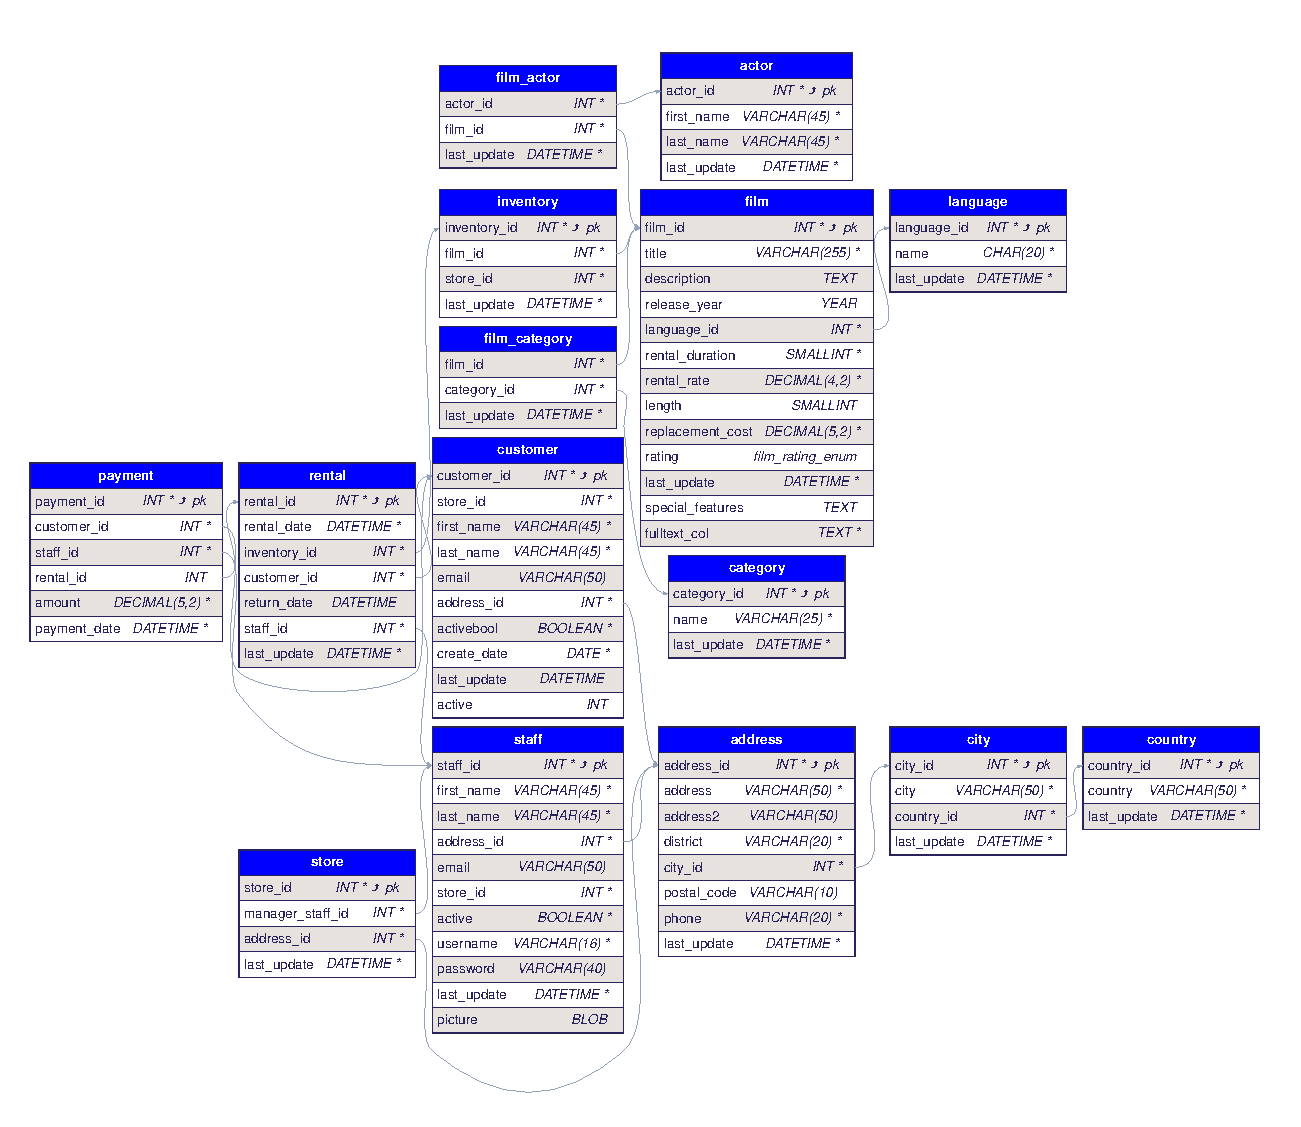
\includegraphics[width=\textheight, height=\textwidth, keepaspectratio, angle=90]{lab_14_schema_cropped.pdf}
\end{figure}
\end{document}